% Este arquivo .tex será incluído no arquivo .tex principal. Não é preciso
% declarar nenhum cabeçalho

\section{Grupos e Entidades da Unicamp}
\subsection{GPSL}

O Grupo Pró Software Livre (GPSL) é aberto para alunos de todos os institutos
e para a comunidade. Seu objetivo é promover o uso e o desenvolvimento do
software livre.

A maioria das instituições educacionais utiliza apenas software
proprietário e a Unicamp não é exceção. São poucos os institutos que usam
software livre e é muito fácil se formar sem sequer saber da existência ou ter
qualquer experiência com algo diferente do software proprietário vigente.

\begin{figure}[h!]
    \centering
    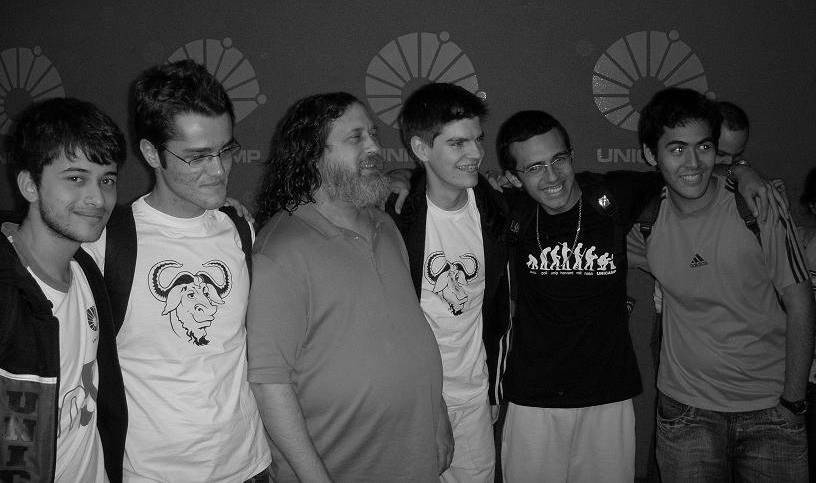
\includegraphics[scale=0.36, keepaspectratio=true]{img/imgs/18-grupos_entidades/stallman2.JPG}
    \caption{Richard Stallman em vista à Unicamp}
\end{figure}
O GPSL é um espaço para refletir sobre este monopólio do software proprietário,
imposto sobre nós através de tantas instâncias, inclusive nossa própria
universidade, a ética (ou falta de ética) por trás disso e seus efeitos sociais.
É também um espaço para se articular e pensar em formas de ação, que podem
envolver desde a educação e conscientização dos usuários de computadores até
o próprio desenvolvimento de software livre. O GPSL também pensa sobre
questões de mercado e econômicas relacionadas ao software livre.

Ultimamente, o GPSL tem sido responsável por organizar, com o apoio do
CACo, o \textbf{Curso de GNU/Linux para os bixos}. Este curso, como o
próprio nome diz, é voltado para os bixos que ingressam nos cursos de
Ciência e Engenharia da Computação (apesar de também ser aberto a todos
os outros alunos dos dois cursos), e tem como objetivo ensinar o
básico do sistema operacional \texttt{GNU/Linux} para você se virar
nas matérias de computação do primeiro semestre. Ele geralmente é
ministrado em abril, mas não existe data fixa. Mas não se preocupe,
algum veterano seu vai passar na sala de aula avisando sobre o curso,
além de sempre avisarmos com antecedência enviando um comunicado ao
seu e-mail do IC.

Para entrar no nossa lista de discussão mande um e-mail para
gpsl-unicamp@googlegroups.com, ou então se cadastre através do site:
\url{groups.google.com/group/gpsl-unicamp}.

\subsection{Gamux}

O Gamux (Grupo de Pesquisa e Desenvolvimento de Jogos da Unicamp), composto por
computeiros e alunos do IA (Instituto de Artes), é uma ótima oportunidade para
quem tiver curiosidade de saber como são feitos os jogos eletrônicos. E isso
tanto de PC quanto console, já que o grupo dispõe de um Xbox para
desenvolvimento.

Mas não espere já chegar fazendo um MMORPG 3D com mais raças que um livro de
Tolkien. Paciência, padawan, você provavelmente começará com algo bem simples,
como um pong, e descobrirá que não é tão simples assim{\dots}

Fique atento, eles costumam organizar um ciclo de palestras semanais sobre como
fazer jogos em XNA (um framework da Microsoft, em C\#, que roda tanto no PC
quanto no Xbox. Sim, bixos sem saber orientação a objetos conseguem acompanhar).

Mas não precisa esperar até lá, apareça no LMS (Laboratório da Microsoft, logo
depois do guarda no IC, é o "beco" na direita) e/ou entre no fórum/lista de
e-mails.

O grupo possui um grande conhecimento em XNA, porque é o mais usado nos inúmeros
concursos que participam (e ganham =), mas, por também ser de pesquisa, não se
restringe a isso. Se você quiser estudar allegro, SDL, Ogre, Game Maker, até
MUGEN (lol), tenha certeza que alguém poderá te ajudar (nem que seja pra te dar
uns links e dizer RTFM).

\begin{itemize}
\item  Site: \url{gamux.com.br}
\item  Lista de discussão: \url{groups.google.com/group/gamedev_unicamp}
\end{itemize}

\subsection{Curso Exato}

O Curso Exato é um projeto da Pró-Reitoria de Extensão e Assuntos
Comunitários da Unicamp criado em 2008 por alunos de graduação, com a
finalidade de explorar o potencial e a capacidade dos alunos de se
expressarem, de raciocinarem logicamente e de compreenderem o mundo que os
cerca, por meio de aulas de Língua Portuguesa, Matemática, Física e Química.

Os professores do curso são alunos de graduação e pós-graduação da
universidade e o público alvo é constituído por alunos da rede pública de
ensino com disposição e interesse para aprender.

As aulas são realizadas no período noturno, das 19h15 às 22h30, de segunda
a sexta-feira, no campus da universidade.

\begin{itemize}
\item  Site: \url{www.cursoexato.com.br}.
\item  E-mail pra contato: curso.exato@gmail.com
\end{itemize}

\subsection{DCE}

Criado em 1978, o DCE (Diretório Central dos Estudantes) é a entidade que
representa todos os estudantes de graduação da universidade, articulando
e organizando o Movimento Estudantil (ME).

Como entidade representativa, cabe ao DCE representar o conjunto dos
estudantes em todos os espaços dentro e fora da universidade, diante das mais
diversas entidades (reitoria, sindicatos, DCEs de outras universidades, Centros
Acadêmicos, associações etc.) e Movimentos Sociais.

Como articulador do ME, cabe ao DCE organizar os estudantes na luta por uma
educação superior realmente pública, gratuita e de qualidade. Para tanto,
é papel fundamental do DCE propor, juntamente com os Centros Acadêmicos,
discussões políticas que extrapolem os nossos currículos e o nosso dia-a-dia.
Além disso, o DCE deve propor ações que vão ao encontro das reivindicações
estudantis, de forma que elas sejam levadas e cobradas da reitoria ou até mesmo
do governo.

O DCE esteve envolvido em várias conquistas dos estudantes, das quais podemos
destacar algumas lutas históricas: A construção da moradia estudantil; a melhora
de estrutura para cursos noturnos (o que tornou acessível para esse período
bibliotecas, xerox, laboratórios e secretarias de graduação); a reunião semestral
para avaliação de curso; o não-aumento do preço do bandejão; uma seleção mais
justa para as vagas na moradia; entre diversas outras. Além disso, o DCE teve
participação em importantes lutas sociais que extrapolam o âmbito da Unicamp,
como a organização do Plebiscito contra a Alca e do Plebiscito contra o Provão;
a luta por mais verbas para a educação no estado de São Paulo; diversas lutas
pela qualidade do ensino e manutenção de direitos dos estudantes em outras
universidades como na UNIP, UNIMEP, FUPPESP etc.

Porém, muitas lutas importantes ainda devem ser travadas por nós estudantes:
Seja por mais bolsas de assistência estudantil, por mais vagas na moradia, por
mais democracia nos espaços de decisão da universidade, por melhorias nos
laboratórios, pela contratação de mais professores etc.

Todo ano (mais precisamente no mês de novembro), há eleições para definir qual
a chapa que comandará a entidade no ano seguinte, assim como há eleições para
representação discente no Consu e na CCG. É muito importante a participação dos
alunos nessas eleições.

Enfim, são muitas as discussões e as lutas que nos aguardam esse ano. Não deixe
de participar da Calourada Integrada (a programação estará espalhada pela
universidade), do DCE (que fica ao lado do Bandejão) e do CACo. Afinal, o ME
deve ser construído por todos nós. Participe!

\begin{itemize}
\item  Telefones: (19) 3521-7910 / 3521-7042.
\item  E-mail: dceunicamp@gmail.com.
\item  Site: \url{www.dceunicamp.org.br}.
\end{itemize}

\subsection{Rádio Muda}

Você provavelmente nunca viu nada do tipo na sua vida. Uma rádio na qual
qualquer ser humano pode fazer o seu programa tranquilamente, sem burocracias
(tendo espaço na grade de horários, lógico).

A Rádio Muda fica embaixo da caixa d'água (carinhosamente apelidada de Pau do
Zeferino) que fica perto do Teatro de Arena, bem em frente à BC (Biblioteca
Central).

Se você só quiser ouvir a muda, 88,5 MHz no seu rádio (em Barão Geraldo ou
Paulínia) ou pela Internet, através do site \url{muda.radiolivre.org}.

\subsubsection{Doidera FM}

O Doidera FM, o programa do doidão, foi fundado em setembro de 2011 por
estudantes de computação e tem por finalidade servir a galera sedenta por
rock'n'roll e loucura pelo menos uma vez por semana. O maior objetivo deste
programa é entreter as pessoas através das ondas eletromagnéticas do rádio na
frequência da Rádio Muda, e também transformar a Rádio Muda em um ponto de
encontro e desencontro, todos os sábados às 23h. Sendo assim, sábado à noite
sabendo ou não o que fazer, cola na Muda para trocar uma ideia, dar muita risada
e curtir muita psicodelia e rock'n'roll.

\subsection{Competições de programação}

\begin{figure}[h!]
    \vspace{-20pt}
    \centering
    
\includegraphics[scale=0.30, keepaspectratio=true]{img/imgs/18-grupos_entidades/maratona.jpg}
    \vspace{-20pt}
\end{figure}
Curte programar? Nunca programou mas está gostando de MC102? Já brincou de
Olimpíada naquelas provinhas com direito a medalha? Vá fundo! Para os bixos
com menos de 20 anos existe a Olimpíada Brasileira de Informática, logo no primeiro
semestre. Anualmente, muitos alunos do IC (em ambos os cursos) ganham premiação
nessa competição. O site dela é \url{olimpiada.ic.unicamp.br}. Esteja
sempre visitando-o.

Ela é uma familiarização para a principal -- a Maratona de Programação (não, não
corremos 40 km programando), que consiste de problemas mais difíceis e é feita
em equipes de 3 alunos. A Unicamp possui uma grande tradição nessa competição,
tendo ido a 4 dos últimos 6 mundiais, e sendo campeã da regional brasileira em
2000, 2002 e 2004. Já houve campeões da Ciência, do mestrado, das duas
modalidades da Engenharia, além de bixos medalhistas. Para maiores informações,
procure pelo site da organização nacional: \url{maratona.ime.usp.br}.
O treinamento com o técnico Alberto Miranda (miranda [@] ic [.] unicamp [.] br)
ocorre às sextas-feiras à tarde no IC-3.

\subsection{Projetos de Extensão Comunitários}
\subsubsection{SUBA}

O SUBA (Sociedade e Universidade em Busca de Alternativas) é um movimento
político surgido em 2003, fruto de uma ocupação de mais de 40 dias ao lado do
bandejão, e que hoje congrega diversos projetos de extensão em debates e ações
acerca do modelo de universidade existente e da possibilidade de transformá-lo.
O SUBA tem uma atuação marcante no questionamento das estruturas da
universidade, se contrapondo à mercantilização da educação impulsionada pelos
cursos pagos, e propõe a construção de uma universidade e de uma sociedade que
vise a superação das desigualdades.

Para conhecer melhor o que é o SUBA informe-se com o pessoal do CACo ou do DCE,
ou vá diretamente ao espaço conquistado que fica ao lado da Praça da Paz.
Conheça também os projetos de extensão comunitátirios (veja o tópico "Grupos
e Entidades da Unicamp"). Segue uma reportagem publicada no CMI (Centro de Mídia
Independente)
\url{www.midiaindependente.org/pt/blue/2003/10/266379.shtml}:

\textit{Estudantes ocupam espaço privatizado na Unicamp}

\textit{Estudantes da Unicamp e movimentos sociais ocuparam, na segunda-feira, dia 20 de outubro, um espaço da universidade desocupado há mais de um ano que tinha sido antes cedido para uma lanchonete Subway e fechado por problemas de higiene e dívidas. Os estudantes e movimentos sociais se reuniram num movimento chamado SUBA (Sociedade e Universidade em Busca de Alternativas) e pretendem dar um uso público e social para o lugar.}

\textit{A reitoria, por sua vez, estuda alugar o espaço para restaurantes, bancos e outras empresas. O espaço está ocupado e uma ampla grade de atividades sociais e culturais foi estabelecida. A programação é aberta e toda a sociedade é convidada a participar das atividades.}

\textit{A ocupação visa a apoiar os debates e a realização de projetos de extensão universitária, atualmente sem o apoio institucional da universidade, além de dar maior visibilidade ao processo de privatização da Unicamp, que vem privilegiando empresas nacionais e transnacionais em detrimento de um ensino público e de qualidade.}

\textit{Apoio: Grupo Aberto de Extensão Universitária; Projetos de Extensão Universitária; Bateria Pública; BioArt; Campanha Nacional contra a ALCA -- Comitê Unicamp; Cinematographo; Comissão de Cultura, Esporte e Lazer do DCE; Diversidade -- Grupo Pela Livre Expressão da Sexualidade Humana; GPSL -- Grupo Pró Software Livre; Grupo de Flautistas; Espaço Cultural da Mogiana/Guanabara; Núcleo pela Reforma Agrária "Carlos Marighella"; Pastoral Universitária; Ponte Pra Lua (Pirofagia); DCE Unicamp -- Diretório Central dos Estudantes; CAB, CACH, CACT, CACo, CAEA, CAECO, CAEF, CALL, CAIA, CAP e outros centros acadêmicos da Unicamp.}

\subsubsection{Cine Clube D'Amora}

Exibe e promove debates de obras fundamentais do cinema na Moradia, com
o objetivo de integração e intercâmbio entre estudantes e moradores dos bairros
vizinhos à Moradia. Que o Cine D'Amora se torne referência para ambos de
cultura, lazer e reflexão!

\subsubsection{Cio da Terra}

Trabalha na perspectiva de uma educação crítica e superadora das desigualdades
sociais na comunidade do Assentamento Rural de Sumaré II. É direcionado aos
moradores locais que concluíram o ensino médio e que querem mas não podem pagar
pela continuidade dos estudos.

\subsubsection{Cursinho da Moradia}

O curso Pré-Vestibular Popular, oferecido na Moradia Estudantil da
Unicamp, é destinado a alunos de baixa renda. Busca propiciar a troca
ativa de conhecimento, não apenas preparando para o vestibular, mas
também estimulando o senso crítico e consciência social dos
estudantes.

\subsubsection{Grupo de Diversidade Sexual}

Grupo de discussão sobre os LGTTBs (Lésbicas, Gays, Travestis, Transexuais
e Bissexuais). Reúne-se às terças-feiras, às 17:30, na cantina do DCE.

\subsubsection{Mano a mano}

Trabalha através da arte-educação com crianças e adolescentes em situação de rua
no centro de Campinas. Objetiva que eles desenvolvam sua autoestima,
reconheçam-se como sujeitos de direitos e questionem a condição em que vivem,
buscando alternativas para sair da rua.

\begin{itemize}
\item  E-mail: manoamano [@] yahoogrupos [.] com [.] br.
\item  Site: \url{move.to/manoamano}.
\end{itemize}

\subsubsection{MAP -- Movimento Abrindo Portas}

Trabalha alfabetização de jovens e adultos excluídos da educação formal em Barão
Geraldo. Objetiva uma alfabetização ampla, da leitura do mundo, contribuindo
para que o educando se reconheça como sujeito de seu aprendizado e da
transformação da sociedade.

\subsubsection{Núcleo Pela Reforma Agrária Carlos Marighella}

O Núcleo desenvolve e participa de atividades político-culturais dentro e fora
da Universidade com o objetivo de discutir as mazelas sociais oriundas do
processo de desenvolvimento da sociedade brasileira e a importância dos
movimentos e organizações populares para a reversão desse quadro, sobretudo no
tocante à questão agrária.

\subsubsection{Projeto Educacional Machado de Assis}

Trata-se de um projeto educacional que funciona no Instituto de Estudos da
Linguagem (IEL). É destinado a estudantes de baixa renda e visa, além do
ingresso destes nas universidades públicas, proporcionar uma formação crítica,
inclusive sobre o próprio caráter excludente do vestibular e da universidade.

\subsubsection{Projeto Educacional Via Popular}

O Via Popular é um projeto de educação popular que, além de abordar conteúdos
programáticos cobrados nos exames de Colégios Técnicos, visa a construção do
senso crítico e o reconhecimento do indivíduo na sociedade e sua capacidade para
transformá-la.

\subsubsection{Sonha Barão}

Junto a disciplina AM018, envolve os alunos da Unicamp no desenvolvimento de
trabalhos sociais em Barão Geraldo, promovendo, assim, a integração da
universidade com a comunidade e proporcionando a vivência da cidadania
e a formação do homem integral.

\subsubsection{Trilharestórias}

Baseado na contação e leitura de histórias, é um projeto de arte-educação que
atua junto a crianças da periferia de Campinas e na Moradia, com o objetivo de
incentivar a imaginação e expressão criativa, além do gosto por histórias, entre
elas as das comunidades que as crianças fazem parte.

\subsubsection{VEJA -- Vivência Educacional de Jovens e Adultos}

Curso de nível fundamental para moradores de Barão Geraldo. Busca o aprendizado
mútuo entre educadores e educandos, através da troca de saberes e de uma
educação reflexiva, dinâmica e prazerosa, que aborde temas da realidade e do
cotidiano.

\subsubsection{Viveiro Guapuruvu}

Por meio da capacitação dos estudantes no trabalho de agro-floresta e realização
de plantios comunitários, busca a articulação dos estudantes com outros setores
da sociedade. Produz mudas em viveiro no IB para o plantio em mutirões no
Assentamento Rural II de Sumaré.

\subsection{Grupos Religiosos}
\subsubsection{Pastoral Universitária}

Grupo católico que se reúne semanalmente para estudar textos (bíblicos ou não),
livros, documentos, aprofundar a fé e promover a integração e união de seus
participantes. A Pastoral Universitária também organiza grupos de preparação
para Primeira Comunhão e Crisma, além de duas Missas semanais e Grupos de Oração
Universitários (GOUs). As Missas são realizadas às terças (18h) e às
quintas (12h15), sempre no PB04. Os GOUs acontecem às terças (12h15) e
nas quintas (18h), também no PB04. Quaisquer dúvidas, acesse o site da
Pastoral (\url{sites.google.com/site/pastoralunicamp/}) ou
envie um e-mail para pastoralunicamp [@] gmail [.] com.

\subsubsection{ABU -- Aliança Bíblica Universitária}

Grupo evangélico não ligado a nenhuma denominação, organiza várias reuniões
e grupos de discussões e é filiado à Aliança Bíblica Universitária do Brasil
(\url{www.abub.org.br}). Quaisquer dúvidas, entre no site
\url{www.abucampinas.org}, mande um e-mail para contato [@] abucampinas
[.] org ou abucamp\_co [@] yahoogrupos [.] com [.] br ou ainda ligue para (19)
3289-2823.

\section{Conpec}

A Conpec é a empresa júnior dos cursos de Ciência e Engenharia da Computação da
Unicamp.
\begin{figure}[h!]
    \vspace{-10pt}
    \centering
    
\includegraphics[scale=0.30, keepaspectratio=true]{img/imgs/19-conpec/logo_bw.png}
    \vspace{-10pt}
\end{figure}
Nela você tem a oportunidade de aplicar os conhecimentos teóricos
adquiridos em sua vida acadêmica em uma situação real, de mercado, com clientes,
prazos e soluções reais. É uma chance ainda de aprender sobre coisas que você
nunca veria na faculdade, como marketing, finanças, planejamento e liderança,
indispensáveis considerando-se que exige-se cada vez mais do profissional de
computação um perfil empreendedor. Muitos ex-membros da Conpec usam os
conhecimentos adquiridos na empresa não só como um adicional ao buscar uma vaga
no mercado de trabalho, mas também para montar suas próprias empresas ou em
serviços não ligados diretamente à computação, como consultorias estratégicas.

Dito isto, a Conpec é uma excelente oportunidade para conhecer os seus colegas
de cursos -- veteranos e bixos, pessoas de outros cursos e até mesmo de fora da
universidade. É ainda uma grande chance para perder a inibição de falar em
público e aperfeiçoar sua capacidade de expor opiniões, além de aprender como
agir em um ambiente profissional.
\begin{figure}[h!]
    \vspace{-10pt}
    \centering
    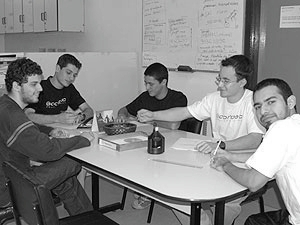
\includegraphics[scale=0.75, keepaspectratio=true]{img/imgs/19-conpec/-101.jpg}
    \vspace{-10pt}
\end{figure}

Para fazer parte da Conpec, fique atento à data da palestra de apresentação do
processo seletivo, que ocorre duas vezes por ano, sempre no início do semestre.
Para saber mais sobre a empresa visite o site \url{www.conpec.com.br} ou
tire suas dúvidas mandando um e-mail para conpec@conpec.com.br.

\section{Atlética -- AAACEC}

Assim como em outras unidades de ensino da Unicamp, o Instituto de Computação
(IC) e a Faculdade de Engenharia Elétrica e de Computação (FEEC) tem sua
entidade que promove a prática de eventos desportivos entre os membros da
graduação e da pós-graduação: A Associação Atlética Acadêmica da Ciência
e Engenharia da Computação, mais conhecida como AAACEC, ou simplesmente
\textbf{Atlética}. A AAACEC é uma entidade sem fins lucrativos, que tem uma
diretoria composta por alunos da computação, eleita a cada ano pelos alunos
dos cursos de Engenharia e Ciência da Computação e pós-graduandos vinculados ao IC.

A AAACEC é a entidade responsável pela participação da Computação em competições
esportivas, tanto dentro da Unicamp (Calouríadas, Interanos, Olimpíadas) como
com faculdades de outras cidades (Intercomp),
\begin{figure}[h!]
    \vspace{-10pt}
    \centering
    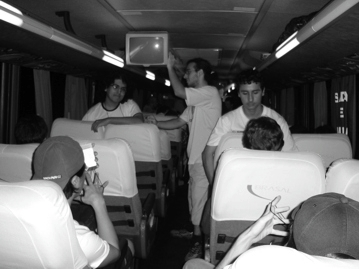
\includegraphics[scale=0.75, keepaspectratio=true]{img/imgs/20-aaacec/-096.jpg}
    \vspace{-10pt}
\end{figure}
competições essas que costumam
acontecer uma vez a cada ano. A fim de possibilitar essa participação, a AAACEC,
além de se encarregar das inscrições e organização, promove treinos regulares de
basquete, vôlei, handball e futsal, e disponibiliza o material (bolas, redes,
etc.) para a prática de tais esportes. A AAACEC se encarrega da reserva e/ou
locação de quadras para a realização dos treinos e competições em que isso se
fizer necessário. Os treinos são semanais e oferecidos para as modalidades
masculina e feminina, de forma que qualquer associado da Atlética pode
participar.

\subsection{Como, então, se associar à AAACEC?}

No caso dos recém-ingressantes, o jeito mais simples é comprando o KIT BIXO,
organizado pela própria AAACEC, contendo camiseta, caneca e outros produtos da
Atlética. Com ele, o calouro torna-se sócio e pode usufruir livremente de todos
os jogos e/ou eventos que a AAACEC venha a organizar pelo resto de sua vida.

Quem não comprar o Kit Bixo no primeiro ano, pode se associar mais tarde com o
pagamento de uma taxa de associação. Além do Kit Bixo, a AAACEC tem diversos
produtos que podem ser comprados por qualquer associado durante todo o curso,
como camisetas, blusas, agasalhos, adesivos, chaveiros, mouse-pads, entre
outros.

\subsection{E para quem vai o dinheiro da compra do kit bixo e dos demais produtos?}

A AAACEC promove a integração entre os alunos, e a realização de experiências
sociais e esportivas:

\begin{itemize}
\item  \textbf{A famosa Choppada Comp/Enf} (gratuita para os bixos)
\item  \textbf{Churrascos}
\item  \textbf{Torneios Esportivos:}
\begin{itemize}
\item  \textit{Internos} (Torneio início, Calouríadas, InterAnos, Olimpíadas)
\item  \textit{Externos} (Intercomp, UniSinos)
\end{itemize}
\begin{figure}[h!]
    \vspace{-10pt}
    \centering
    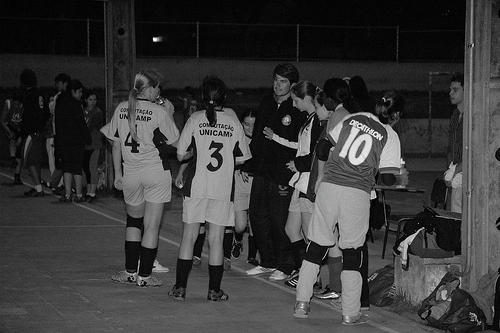
\includegraphics[scale=0.58, keepaspectratio=true]{img/imgs/20-aaacec/-100.jpg}
    \vspace{-10pt}
\end{figure}
\item  \textbf{Festas} (Muitas delas em união com outros cursos, promovendo ainda maior integração)
\end{itemize}

Para tudo isso, é necessário capital, que é obtido com muito trabalho da
Diretoria com a venda dos Kits Bixo e produtos.

É importante lembrar que a diretoria não tem remuneração alguma: Os diretores
trabalham pelo ideal comum de fazer a Computação crescer, e, consequentemente,
ganhar experiência de organização de eventos e pessoas, aprendizado de valor
inestimável, tanto na vida profissional como social.

A AAACEC busca fortalecer, acima de tudo, o nome do curso de Computação da
Unicamp, enaltecendo nossas qualidades dentro e fora da Universidade! Orgulho de
ser Computação Unicamp!!

Faça parte você também dessa integração! Associe-se à AAACEC!

As diretorias anteriores da AAACEC podem ser vistas em:
\url{aaacec.com/diretoria}

\subsection{Contato}

Não hesite em tirar dúvidas ou enviar sugestões!

\begin{itemize}
\item  E-mail: aaacec@ic.unicamp.br
\item  Site: \url{aaacec.com}
\end{itemize}

\subsection{Atendimento}

Ainda não há uma definição para este semestre, mas provavelmente o atendimento
será de segunda a sexta das 12h30m às 13h30m e segunda a quinta das 18h-19h

\subsection{Reuniões}

As reuniões serão marcadas no começo do semestre. Elas são realizadas num dia
letivo às 12h no IC-3.

\subsection{Bateria Valorosa}

Criada em 1998, a bateria Valorosa é umas das melhores baterias da Unicamp.

Durante o ano, ela participa de diversos eventos, como o Intercomp, Interbatuc,
UPA, e apoiando nossos atletas em jogos internos. Também somos convidados por
outros cursos para tocar em seus jogos.

A Bateria realiza ensaios semanais, dos quais estão todos convidados a
participar.

Esperamos que muitos bixos participem, e para isso basta comparecer aos ensaios,
lembrando que não é necessário saber tocar nenhum instrumento. TODOS que
quiserem aprender serão muito bem-vindos na bateria!

\section{Centro Acadêmico da Computação}

Vulgo CACo, é uma entidade autônoma e sem fins
lucrativos, formada por estudantes de graduação dos cursos de Engenharia
e Ciência da Computação e pós-graduação do IC, com o objetivo principal de
representar esses estudantes no âmbito acadêmico. Todo aluno desses cursos é um
membro do CACo.

Já ouviu falar em movimento estudantil? Então{\dots} É nóis!
\begin{figure}[h!]
    \vspace{-10pt}
    \centering
    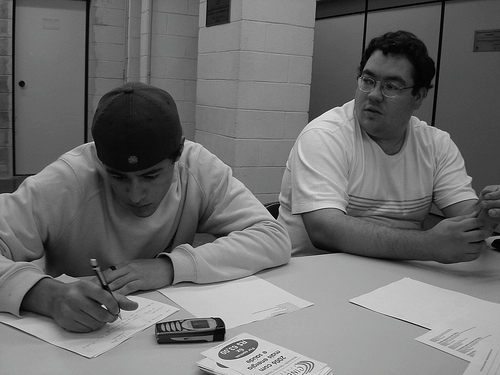
\includegraphics[scale=0.58, keepaspectratio=true]{img/imgs/21-CACo/-123.jpg}
    \vspace{-10pt}
\end{figure}

Como o CACo representa os estudantes? Por exemplo, fazendo este utilíssimo
Manual do Bixo, de qualidade inigualável, inquestionável e inconteste, que tem
a pretensão de ajudá-lo neste começo de vida universitária. Tudo bem, o que
mais? Ajudamos a melhorar a qualidade dos nossos cursos através do GDA (Grupo
Discente de Avaliação), e fomentamos discussões com palestras e mesas redondas
com convidados especialistas. Realizamos assembleias com um número maior de
alunos para tomar decisões mais polêmicas e delicadas, reivindicamos espaço
físico decente para o lazer e a convivência entre os estudantes e promovemos
eventos de integração e discussão, como o CineCACo e o PipoCACo. Procuramos
facilitar a vida dos estudantes, instalando uma máquina de refrigerante
e guloseimas, e também um orelhão na entrada do IC-3. 
Essas são algumas das atividades realizadas pelo CACo, e que serão explicadas
com maiores detalhes mais adiante.

O CACo é o seu centro acadêmico, então nos procure quando você tiver algum
problema, reclamação ou sugestão para o IC ou para a FEEC que o CACo irá te dar todo
o suporte necessário. Dentro do nosso alcance, daremos as informações de que você
precisar, conversaremos com professores, ou até com o diretor do Instituto,
caso seja preciso, assim como se você tiver alguma sugestão ou reclamação com
relação ao CACo. Portanto, não tenha medo de falar conosco!

\begin{itemize}
\item  E-mail: caco@ic.unicamp.br
\item  Site: \url{www.caco.ic.unicamp.br}
\item  Reuniões: você será informado no começo do semestre sobre os horários das reuniões. Participe!
\end{itemize}

Veja abaixo alguns dos projetos que o CACo participa ou realiza.

\subsection{Representação discente}

O CACo tem representantes discentes ativos nos três órgãos colegiados (CI, CG e
Congregação) do IC e da FEEC. Todas as discussões levantadas nesses órgãos que
dizem respeito aos alunos são repassadas nas reuniões ordinárias do Centro Acadêmico.

\subsection{Reunião de avaliação de curso}

A reunião de avaliação de curso também é uma conquista dos estudantes da
Unicamp. Essa reunião acontece uma vez a cada semestre, geralmente
nos meses de maio (primeiro semestre) e outubro (segundo semestre),
numa terça ou quinta-feira, no horário das 10h às 12h para os cursos
diurnos/integrais e das 19h às 21h para os cursos noturnos. Durante esses
horários, os alunos estão dispensados das aulas.

Nas nossas reuniões de avaliação, participam os alunos, os coordenadores de curso e alguns
professores, além de responsáveis pela infraestrutura do IC e da FEEC. Nessas
reuniões são feitas análises sobre o curso, avaliações a respeito de disciplinas,
da infraestrutura de informática e demais discussões (encontrar
deficiências e propor soluções) para que se possa melhorar os
cursos.

Os alunos têm um papel muito importante nessas reuniões, já que são eles os
principais e maiores interessados pelo que pode sair dessas reuniões.

\subsection{Reforma Curricular}

Na Unicamp, os catálogos dos cursos (conjunto de matérias que os compõem)
são atualizados ano a ano. Faz parte da nossa atenção constante identificar falhas
e propor melhorias no nosso currículo.

Reformas curriculares são muito importantes, por manter o curso mais atualizado,
dentro dos padrões do que o mercado e as novas tecnologias exigem. Consulte o seu
catálogo em \url{www.ic.unicamp.br/cg/catalogos-de-graduacao}.

\subsection{Caravana para o fisl}

O fisl (Fórum Internacional Software Livre) ocorre todo ano em Porto Alegre.
É um dos maiores da categoria, reúne milhares de pessoas do mundo todo e conta
com palestras dos mais renomados nomes da computação. E é claro que os
computeiros da Unicamp não podem ficar de fora!
\begin{figure}[h!]
    \vspace{-10pt}
    \centering
    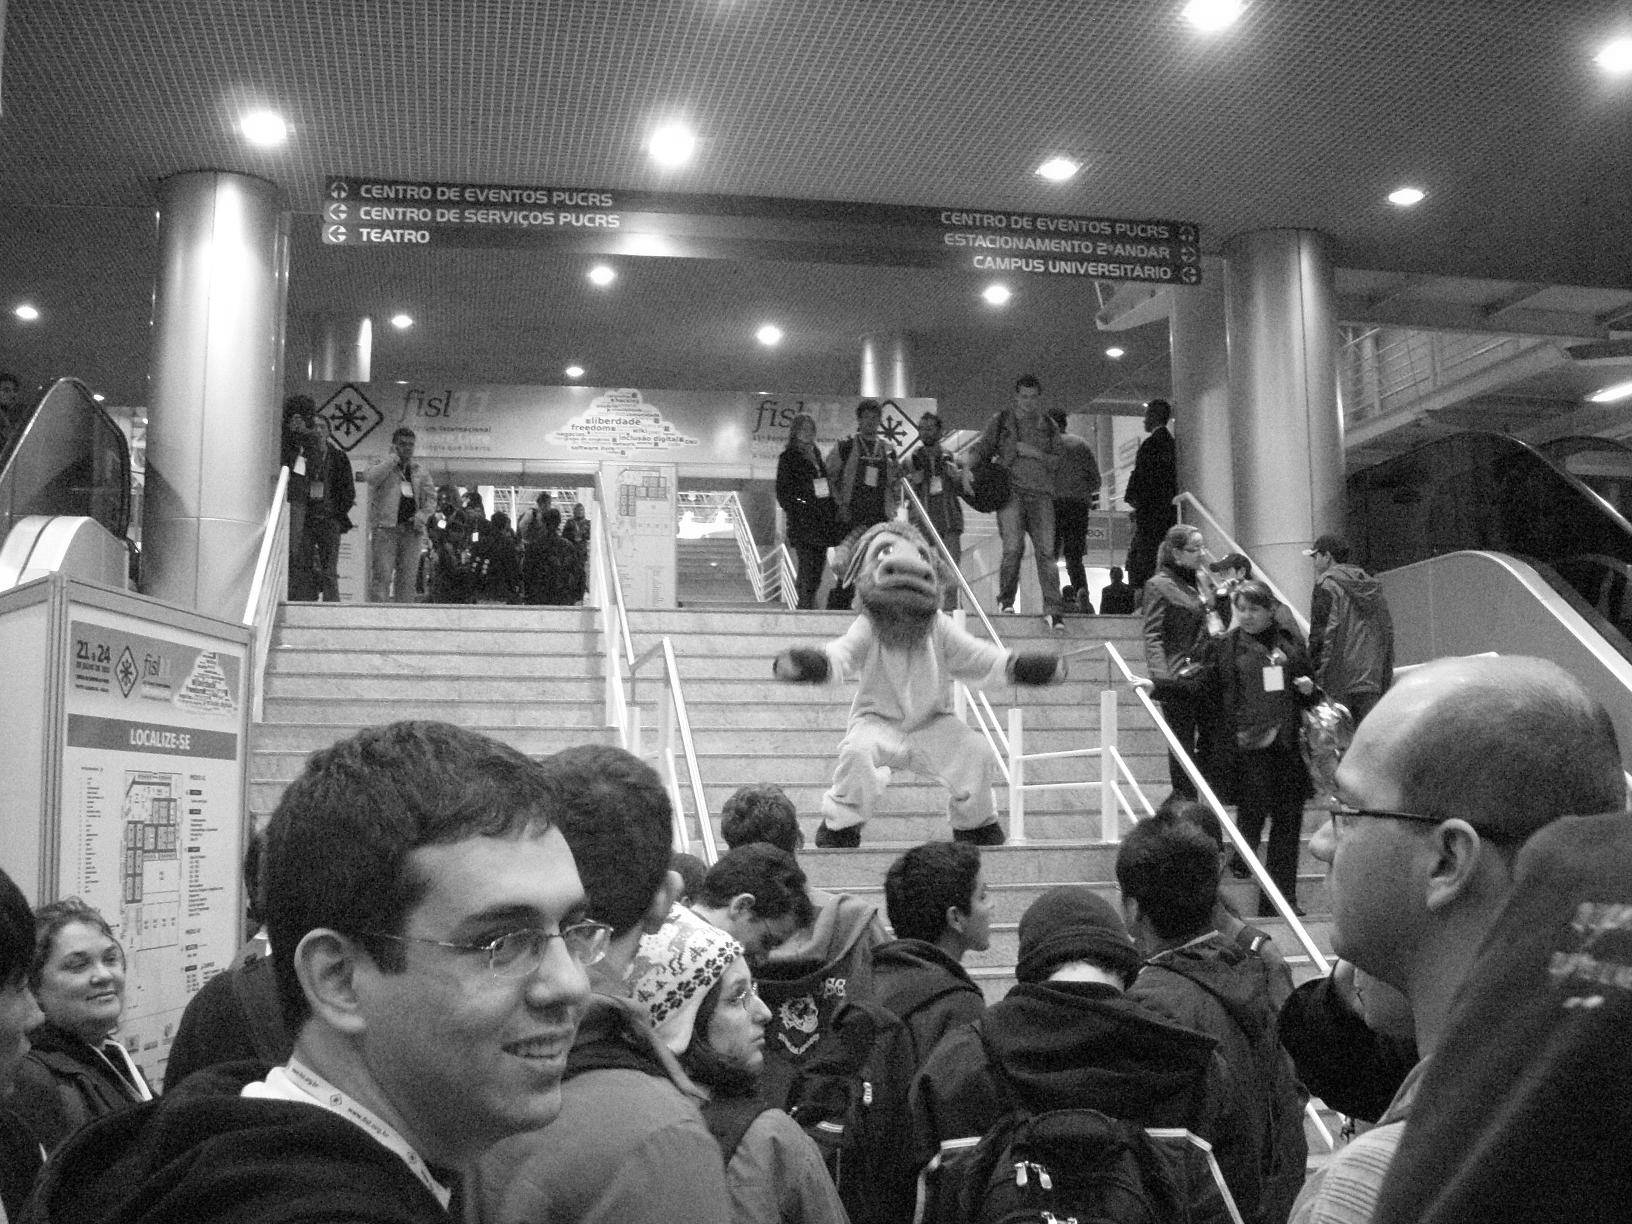
\includegraphics[scale=0.58, keepaspectratio=true]{img/imgs/21-CACo/fisl11_1.jpg}
    \vspace{-10pt}
\end{figure}
O CACo organiza todo ano uma
caravana para o Fórum. Com o patrocínio dos institutos, nós conseguimos fazer
a caravana mais barata de todo fisl. Mesmo para quem acabou de entrar, o fórum
é uma ótima oportunidade para entrar em contato com o mundo da computação.

\subsection{Pesquisa Salarial}

Em 2010, com a colaboração do diretor do IC, o professor Hans Liesenberg,
e da rede social Reunion, promovemos uma pesquisa salarial com
ex-alunos de computação, que ajudou a fornecer um bom panorama da realidade em que se encontra
o profissional formado pela Unicamp na área de computação. A pesquisa
está disponível no site do CACo.

\subsection{CineCACo}

Filme. No IC. Pipoca e refrigerante incluídos.

\subsection{PipoCACo}

O PipoCACo é um espaço de discussão do CACo, onde vários computeiros se reúnem
para discutir um tema de interesse (discussões sobre universidade pública,
eleições, reforma curricular e trote, por exemplo), sempre regado a pipoca
e refrigerante.

Esse espaço também é utilizado para guiar o CACo nas decisões a serem tomadas,
como, por exemplo, o que os alunos defendereriam frente à Coordenadoria de
Graduação, acerca de reforma curricular.

O PipoCACo é um ótimo momento para os bixos se conhecerem e também
conhecerem as atividades do CACo de forma mais descontraída.

\subsection{Palestra Azoide/Bzoide}

A Palestra Azoide/Bzoide é um evento em que professores, alunos e ex-alunos expõem
e discutem as modalidades AA e AB da Engenharia de Computação. A palestra vem se mostrando muito importante
para a definição de qual modalidade seguir, principalmente por desmentir grandes
mitos. O principal deles é aquele que diz que AA é somente software e AB
é somente hardware. A palestra é destinada aos alunos da Engenharia,
já que a Ciência conta com apenas uma modalidade de curso.
\begin{figure}[h!]
    \vspace{0pt}
    \centering
    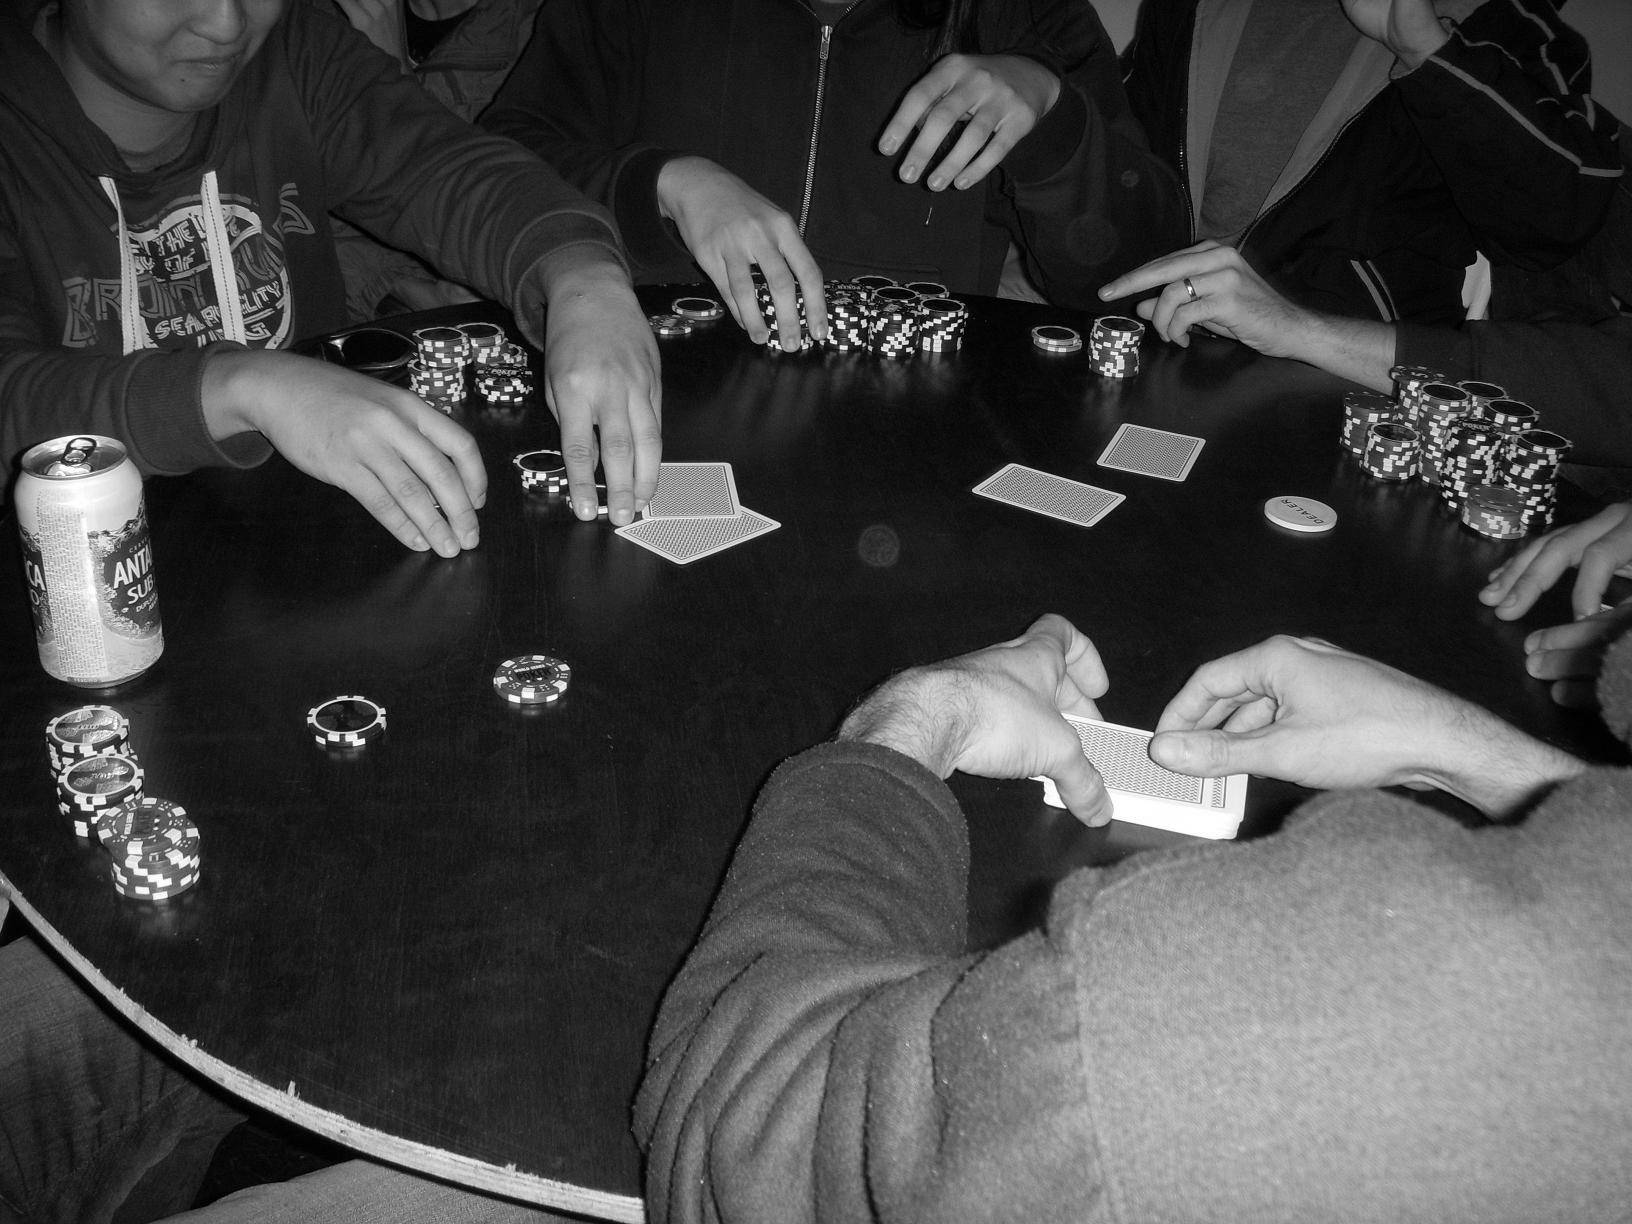
\includegraphics[scale=0.55, keepaspectratio=true]{img/imgs/21-CACo/poker.jpg}
    \vspace{-10pt}
\end{figure}


\subsection{CACo Series of Poker}

Semestralmente, o CACo organiza um torneio de poker para os alunos,
possibilitando grande integração da galera. Você será informado da data de
realização do próximo torneio! Fique atento.

\subsection{Listas de e-mail do CACo}

As listas de e-mail do CACo são listas de discussão dos alunos de computação da
Unicamp que visam a integrar os computeiros de vários anos, fomentar discussões
ou debater ideias e posições do CACo em relação aos assuntos de interesse dos
alunos que representa.

Atualmente, o CACo conta com três listas de discussão com objetivos distintos:

\begin{itemize}
\item  \textbf{Computeiros (computeiros@caco.ic.unicamp.br)}: Lista de todos as turmas de computação. Tem por objetivo integrar todos os alunos. É o lugar onde se pode pedir dicas de matérias, opiniões sobre os melhores professores para cada matéria, trocar informações e se confraternizar.
\end{itemize}

\begin{itemize}
\item  \textbf{Gestão (gestao [@] caco [.] ic [.] unicamp [.] br)}: Discussões ligadas estritamente à gestão do Centro Acadêmico.
\end{itemize}

\begin{itemize}
\item  \textbf{Offtopic (offtopic [@] caco [.] ic [.] unicamp [.] br)}: A lendária lista para discussões infinitas sobre qualquer assunto, de política, ciência e religião a Filme do Bátima.
\end{itemize}

Para participar das listas, visite a página das listas do CACo:
\url{sardinha.caco.ic.unicamp.br}.

\subsection{Atendimento}

O CACo disponiliza um horário para que que você possa comprar algum de nossos
produtos, tirar dúvidas ou apenas se comunicar conosco. Para conferir nossos
horários de atendimento, visite o site do CACo.


\subsection{Gestão}

A atual gestão do Centro Acadêmico foi eleita no fim de novembro de 2011 e deve
se prolongar até outubro deste ano. Mas lembre-se: o CACo não é formado só por
seus coordenadores. O coletivo de nosso Centro Acadêmico é bem maior. Lembre-se
de que todo estudante de Computação tem o direito de dar pitaco nas discussões
do CACo. Os calouros sempre realizam funções decisivas no Centro Acadêmico.

Para ficar mais integrado ao que ocorre no seu Centro Acadêmico, como as suas
ações, projetos e quais os problemas atuais, você pode se increver na lista da
gestão do CACo através do site das listas de discussão do CACo:
\url{sardinha.caco.ic.unicamp.br}

Portanto, não tenha medo! Tenha vontade! Venha participar e construir o nosso
Centro!
\begin{figure}[t!]
    \centering
    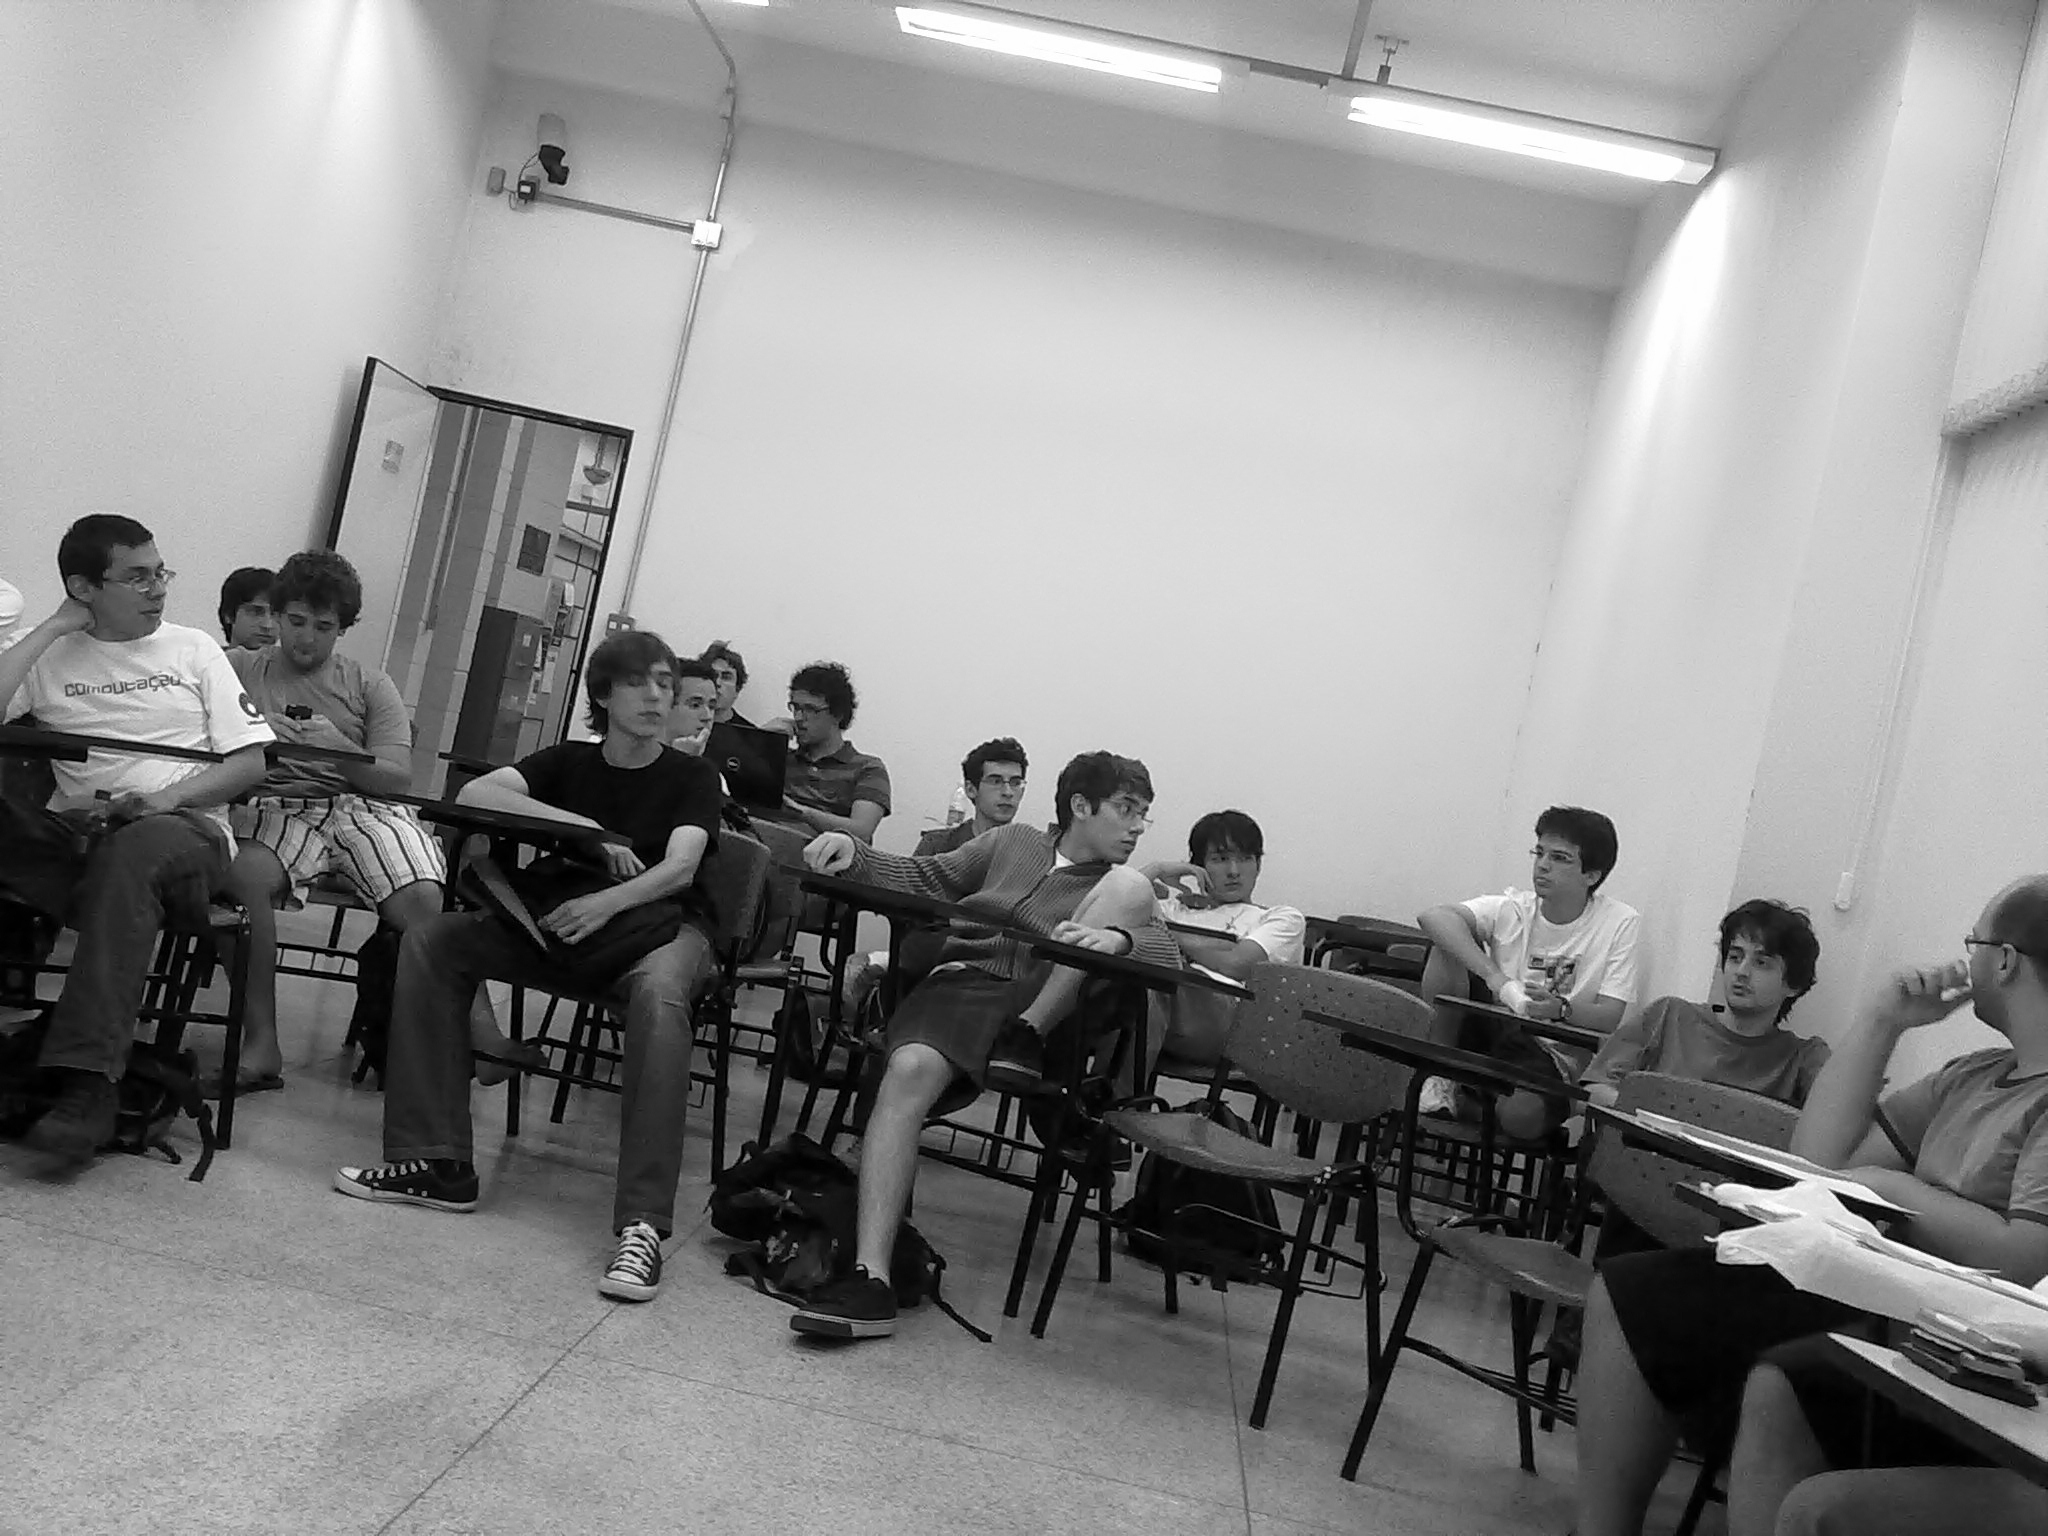
\includegraphics[scale=0.47, keepaspectratio=true]{img/imgs/21-CACo/reuniao.jpg}
\end{figure}


\subsubsection{Chapa "Não é fácil ser verde" (2011/2012)}

\begin{itemize}
\item  \textbf{Presidência}
\begin{itemize}
\item Thiago Rosario Caetano (Thiago EC010)
\end{itemize}
\end{itemize}

\begin{itemize}
\item  \textbf{Coordenadoria Administrativa}
\begin{itemize}
\item Humberto Aboud Torres Lobo (Sheldon EC010) 
\end{itemize}
\end{itemize}

\begin{itemize}
\item  \textbf{Coodenadoria Financeira}
\begin{itemize}
\item  André Felipe Barros Selva (Selva EC09)
\item  Rafael Kümmel (Chaminé EC011)
\end{itemize}
\end{itemize}

\begin{itemize}
\item  \textbf{Coordenadoria de Ensino e Graduação}
\begin{itemize}
\item Raphael de Oliveira Costa Danella (Danella EC08)
\item Victor Fernando Pompêo Barbosa (Pompêo EC09)
\item Pedro Henrique Azevedo Amorim (Amorim EC011)
\end{itemize}
\end{itemize}

\begin{itemize}
\item  \textbf{Coordenadoria de Ensino e Pós-Graduação}
\begin{itemize}
\item Alex Bredariol Grilo (Alex CC07)
\end{itemize}
\end{itemize}

\begin{itemize}
\item  \textbf{Coordenadoria de Comunicação}
\begin{itemize}
\item  Gérson de Paulo Carlos (Gérson EC09)
\end{itemize}
\end{itemize}

\begin{itemize}
\item  \textbf{Coordenadoria de Eventos e Cultura}
\begin{itemize}
\item José Américo Nabuco Leva Ferreira de Freitas (Jota EC010)
\item Wesley T. S. T. Ide (Wesley CC010)
\item Júlia Ramos Beltrão (Júlia EC011)
\end{itemize}
\end{itemize}

\begin{itemize}
\item  \textbf{Coordenadoria de Marketing}
\begin{itemize}
\item Fernando Bastos Lucchesi Jurema (Tomitinha EC09)
\item Guilherme Rolfsen Franzoni (Guegs EC010)
\item Victor Rodrigues Matsuguma (Preciso EC011)
\end{itemize}
\end{itemize}

\begin{itemize}
\item  \textbf{Coordenadoria de Produtos}
\begin{itemize}
\item Vinícius Pimental Couto (Auschwitz EC011)
\item Tiago Lobato Gimenes (Bassi EC011)
\end{itemize}
\end{itemize}

\begin{itemize}
\item  \textbf{Coordenadoria Tecnológica}
\begin{itemize}
\item Alexandre Novais de Medeiros (Salsicha CC011)
\item Gabriel Hidasy Rezende (Sam EC011)
\end{itemize}
\end{itemize}

\begin{itemize}
\item  \textbf{Coordenadoria de Patrimônio}
\begin{itemize}
\item Wesley Dias (Kiabbo EC010)
\item Pedro Gabriel Calixto (Transitions EC011)
\end{itemize}
\end{itemize}

As gestões anteriores do CACo podem ser vistas em:
\url{www.caco.ic.unicamp.brinstitucional/gestões}
